\documentclass[11pt]{article}
\usepackage[margin=2.3cm]{geometry}
\usepackage{amsmath,amssymb,amsthm,mathtools}
\usepackage{enumitem}
\usepackage{tikz}
\usepackage{hyperref}
\usetikzlibrary{positioning,arrows.meta,calc}
\theoremstyle{definition}
\newtheorem{definition}{Definition}
\theoremstyle{plain}
\newtheorem{proposition}{Proposition}
\newtheorem{theorem}{Theorem}
\newtheorem{conjecture}{Conjecture}
\theoremstyle{remark}
\newtheorem{remark}{Remark}
\newcommand{\Hol}{\operatorname{Hol}}
\newcommand{\Spin}{\mathrm{Spin}}
\newcommand{\Z}{\mathbb{Z}}
\newcommand{\R}{\mathbb{R}}
\title{\textbf{Gauge-Theoretic Signed-Hypergraph Learning}\\[2pt]
\large HSiKAN fibers, rotor connections, spike-walk holonomy, and the semiring convolution that unifies them}
\author{Aiko --- for Dr.\ Cs.\ Hajdu \& Prof.\ Kato}
\date{2026-06-25 \quad(technical report; conjectures marked as such)}
\begin{document}
\maketitle
\begin{abstract}
We develop a gauge-theoretic account of computation on signed hypergraphs and use it to organise --- and extend ---
the HSiKAN line. Three claims structure the report. (i) Every computation HyMeKo performs over its signed
hypergraph is a \emph{semiring convolution} of the signed incidence with a vertex field; the choice of semiring
(additive, tropical, parity, fuzzy, spinor) is the choice of computational regime, and we give the conditions
under which it is well defined. (ii) The \emph{signal} that signed-link prediction exploits --- structural balance
--- is exactly a \emph{holonomy}: signs are a $\Z_2$ connection and balance is its trivial holonomy. (iii) HSiKAN
is naturally read as a learned \emph{section} of a fiber bundle over the hypergraph; a \emph{rotor} (a $\Spin$
element) on each arc is a \emph{connection} that parallel-transports those learned fibers; \emph{spike-walks}
(the tropical/event reading) time the transport; and the \emph{spiral collects the transported fibers at the
walk ends}, computing a learned, continuous holonomy that \emph{strictly generalises the balance parity}. This
predicts a concrete, falsifiable way the construction could lift AUROC --- distinct from the rotor-as-readout
experiment already settled in the negative --- and simultaneously opens an event-based (neuromorphic) regime and a
structural debuggability we have already built. We state the mathematics, the architecture, the testable claims,
and an honest scope (theorem vs.\ conjecture vs.\ engineering).
\end{abstract}

\tableofcontents

\section{Motivation: why a gauge picture}
HSiKAN (Highway Signed KAN) has, on serial-chain control and on Bitcoin-OTC signed-link prediction, \emph{tied} a
parameter-matched MLP / B-spline baseline. Two readings are possible: ``the structural prior is inert'' or ``the
prior was tested where the structure carries no exploitable signal.'' This report argues the second, and makes it
precise: the predictive content of a signed (hyper)graph is \emph{gauge-theoretic} --- it lives in the
\emph{holonomy} of a connection, not in node features --- so a method only benefits when (a) the topology has
non-trivial holonomy to read (cycles, frustration, branching) and (b) the architecture actually computes a
holonomy rather than a pooled feature. We show HSiKAN supplies a learned fiber, a rotor supplies a connection,
spikes supply the timing, and the three compose into a holonomy readout that is the natural continuous lift of the
balance invariant.

\section{Preliminaries}
\subsection{Signed hypergraph and incidence}
A \emph{signed weighted hypergraph} is $H=(V,E,w,\sigma)$, $|V|=n$, $|E|=m$, with arc weights $w_{ev}\in\R$ and
signs $\sigma_{ev}\in\{\pm1\}$ for $v\in e$. Its star-expansion promotes each hyperedge to a hub and yields the
\emph{signed incidence} $B\in\R^{n\times m}$, $B_{ve}=\sigma_{ev}w_{ev}$ if $v\in e$ else $0$. $B$ is the discrete
boundary $\partial:C_1\!\to\!C_0$ of the chain complex; $B^{\!\top}$ the coboundary $\delta$.

\subsection{Fiber bundles, connections, holonomy (discrete)}
\begin{definition}[Discrete $G$-bundle and connection]
Let $G$ be a group (the \emph{structure group}) acting on a fiber $F$. A \emph{discrete $G$-connection} on the
graph assigns to each oriented arc $u\!\to\!v$ an element $g_{uv}\in G$ with $g_{vu}=g_{uv}^{-1}$. A
\emph{section} assigns to each vertex a fiber element $h_v\in F$. \emph{Parallel transport} of $h_u$ along
$u\!\to\!v$ is $g_{uv}\!\cdot\!h_u$.
\end{definition}
\begin{definition}[Holonomy]
For a walk $W=(v_0,\dots,v_k)$ the \emph{transport} is $\Hol(W)=g_{v_{k-1}v_k}\cdots g_{v_0v_1}\in G$. For a
closed walk (cycle) $\Hol(W)$ is the \emph{holonomy}; it is invariant under \emph{gauge transformations}
$g_{uv}\mapsto s_v\,g_{uv}\,s_u^{-1}$ for any vertex relabelling $s:V\to G$ (up to conjugacy).
\end{definition}

\subsection{Rotors (Clifford / Spin)}
In the Clifford algebra $\mathrm{Cl}(\R^d)$ a \emph{rotor} $R=e^{\tfrac12\theta\,\hat B}$ ($\hat B$ a unit
bivector) is an even, unit-norm element; $R\in\Spin(d)$ acts on a vector $x$ by the sandwich $x\mapsto R x R^{-1}$,
a rotation by $\theta$ in the plane $\hat B$. Rotor composition (the geometric product) is associative,
unit-bearing ($R=1$), and \emph{non-commutative} for $d\ge 3$ --- the property that lets an ordered product encode
order.

\section{The semiring convolution (the computational substrate)}
\begin{definition}[Aggregation algebra]
A commutative monoid $(S,\oplus,\mathbf0)$; for signed-weighted aggregation a semiring
$(S,\oplus,\otimes,\mathbf0,\mathbf1)$ with $\otimes$ distributing over $\oplus$ and $\mathbf0$ annihilating.
\end{definition}
\begin{definition}[Convolution]
For a field $x\in S^V$, $(B\circledast x)_e=\bigoplus_{v\in e}\sigma_{ev}w_{ev}\otimes x_v$ --- the semiring
matrix--vector product.
\end{definition}
\begin{proposition}[Well-definedness]\label{prop:wd}
$(B\circledast x)_e$ is order-independent over the unordered members of $e$ iff $\oplus$ is commutative and
associative; defined on empty/masked members iff $\oplus$ has identity; composable across nesting iff $\otimes$
distributes over $\oplus$. Hence a tag is admissible iff it names a commutative monoid (semiring for
signed-weighted).
\end{proposition}
\begin{remark}[Ordered walks vs.\ unordered members]\label{rem:order}
A hyperedge's members are unordered, so the cross-member fold needs a \emph{commutative} $\oplus$. A
\emph{walk} is ordered, so transport along it is a chain of $\otimes$; there $\otimes$ \emph{may be
non-commutative} (a rotor) and this is desirable --- it encodes walk order. The two never conflict:
commutativity is required only of $\oplus$.
\end{remark}

\paragraph{Catalog of regimes.} additive $(\R,+,\times)$ --- the graph Laplacian / linear message passing;
parity $(\{\pm1\},\times)$ --- Cartwright--Harary balance; tropical $(\R\cup\{\infty\},\min,+)$ --- event/spike
timing; fuzzy $([0,1],\bot,\top)$ --- residuated, single-layer unless distributive; \textbf{spinor}
$(\Spin,\ \oplus,\ \text{geometric product})$ --- the connection/transport regime developed below.

\section{Signed graphs are $\Z_2$ gauge fields; balance is holonomy}
\begin{theorem}[Balance as trivial holonomy]\label{thm:balance}
Take $G=\Z_2=\{\pm1\}$ with the sign $\sigma_{uv}$ as the connection. A signed graph is \emph{balanced}
(Cartwright--Harary: every cycle has an even number of negative edges, i.e.\ $\prod_{e\in C}\sigma_e=+1$) iff its
$\Z_2$ holonomy is trivial, $\Hol(C)=+1$ for every cycle $C$; equivalently iff the connection is gauge-equivalent
to the all-$+1$ connection ($\exists\,s:V\to\{\pm1\}$ with $s_u\sigma_{uv}s_v=+1$).
\end{theorem}
\begin{proof}[Sketch] $\Hol(C)=\prod_{e\in C}\sigma_e$ is the product of signs around $C$; gauge transformations
cancel in pairs around any closed walk, so $\Hol$ is gauge-invariant, and $\Hol\equiv+1$ on a spanning set of
cycles is exactly solvability of $s_u\sigma_{uv}s_v=+1$ on a spanning tree extended by the cycle constraints. \end{proof}
\begin{remark}[Where the AUROC signal lives]
Real signed graphs are \emph{frustrated}: $\Hol(C)\ne+1$ on some cycles. Signed-link prediction is precisely the
problem of inferring an edge's sign from the holonomy of surrounding cycles; the \emph{frustration} (deviation of
$\Hol$ from $+1$) is the residual signal beyond a globally balanced fit. Any predictor is, implicitly, estimating
holonomy.
\end{remark}

\section{The Spin lift: from $\Z_2$ to a learned continuous holonomy}
Replace $G=\Z_2$ by $G=\Spin(d)$ (or $U(1)$/$SU(2)$): each arc carries a \emph{rotor} $R_{uv}\in\Spin$, a
\emph{learned} connection, and $\pi:\Spin\to\Z_2$ (e.g.\ the sign of a fixed scalar component, or restriction to
$\{\pm1\}\subset\Spin$) recovers the discrete sign.
\begin{proposition}[The Spin holonomy refines balance]\label{prop:lift}
Under $\pi:\Spin\to\Z_2$, $\pi(\Hol_{\Spin}(C))=\Hol_{\Z_2}(C)=\prod_{e\in C}\sigma_e$. Thus the rotor holonomy
$\Hol_{\Spin}(C)\in\Spin$ is a continuous invariant whose $\Z_2$ projection is exactly the balance parity; it
carries strictly more information (a rotation angle / bivector plane), and it is gauge-covariant.
\end{proposition}
\begin{remark}
$\Hol_{\Spin}$ is the discrete \emph{curvature} (Wilson loop) of the learned connection: balanced cycles give
$\Hol_{\Spin}\!\approx\!1$, frustrated cycles give a non-trivial rotation whose magnitude grades the frustration.
This is the object we propose to feed the predictor --- a learned, continuous generalisation of the exact balance
signal.
\end{remark}

\section{HSiKAN is the fiber; the rotor is the connection}
\begin{definition}[HSiKAN section]
HSiKAN's per-vertex output $h_v\in\R^{d}$ (the \texttt{node\_activations} before pooling) is a learned section of
the bundle: a Catmull-Rom--activated, highway-gated, signed-conv aggregation. Stacking layers is a learned
\emph{covariant} aggregation (message passing along $B$).
\end{definition}
The construction has two stages, deliberately separated (this is what distinguishes it from the settled
rotor-as-readout experiment):
\begin{enumerate}[nosep,leftmargin=1.4em]
  \item \textbf{Fiber (HSiKAN):} learn rich per-vertex representations $h_v$ --- the heavy representational work.
  \item \textbf{Connection (rotor):} transport those fibers along walks via $R_{uv}$; \emph{collect the
        transported fibers at the walk ends}; the readout consumes $\Hol_{\Spin}(W)\!\cdot\!h$, not raw signs.
\end{enumerate}

\section{Walk-spikes: the tropical timing of the transport}
Read arc weights as \emph{delays}: the tropical semiring $(\min,+)$ computes the \emph{earliest spike arrival}
along signed walks; a walk $W$ emits a spike at $\tau_W=\sum_{e\in W}w_e$ carrying its parity (and, in the Spin
lift, its rotor $\Hol_{\Spin}(W)$). A depth-$k$ stack is a leaky-integrate-and-fire pass with structural delays.
\begin{remark}[Why timing matters here]
The spike \emph{gates which transport reaches the head first}: the tropical $\min$ selects the \emph{shortest}
signed walk, and short walks accumulate less sign noise, so the earliest-spike readout is a principled
``trust the shortest balanced path'' bias. Idempotence $a\oplus a=a$ makes the representation sparse and
event-driven --- the neuromorphic / embedded regime, and the natural form of the \emph{fast reflex} in the
rate-asymmetric controller.
\end{remark}

\section{The synthesis: the spiral collects fibers at spike-walk ends}
\begin{figure}[h]\centering
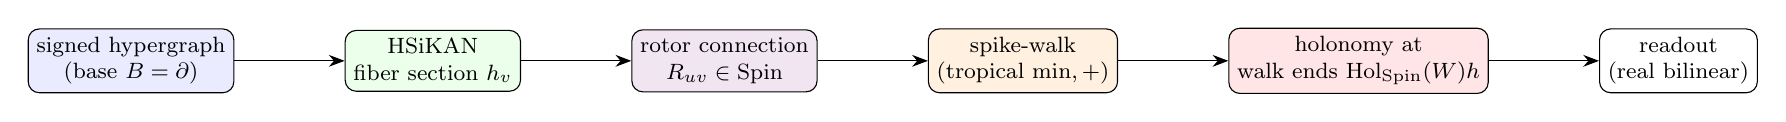
\begin{tikzpicture}[font=\footnotesize,>={Stealth[length=2mm]},node distance=8mm and 14mm,
  b/.style={draw,rounded corners,align=center,inner sep=3pt}]
  \node[b,fill=blue!8] (hg) {signed hypergraph\\ (base $B=\partial$)};
  \node[b,fill=green!8,right=of hg] (fib) {HSiKAN\\ fiber section $h_v$};
  \node[b,fill=violet!10,right=of fib] (conn) {rotor connection\\ $R_{uv}\in\Spin$};
  \node[b,fill=orange!12,right=of conn] (spike) {spike-walk\\ (tropical $\min,+$)};
  \node[b,fill=red!10,right=of spike] (hol) {holonomy at\\ walk ends $\Hol_\Spin(W)h$};
  \node[b,right=of hol] (head) {readout\\ (real bilinear)};
  \draw[->](hg)--(fib); \draw[->](fib)--(conn); \draw[->](conn)--(spike);
  \draw[->](spike)--(hol); \draw[->](hol)--(head);
\end{tikzpicture}
\caption{HSiKAN learns the fiber; the rotor connection transports it; spikes time the transport (shortest signed
walk first); the spiral collects the parallel-transported fibers at the walk ends; a fixed real-bilinear head
scores. The new signal is the \emph{transport/holonomy}, with the readout held at the algebra already shown best.}
\end{figure}
The edge $(u,v)$ is scored from the holonomy-transported fibers along $u\!\to\!v$ walks,
\[
\hat y_{uv}=f_{\text{bilinear}}\!\Big(\bigoplus_{W:\,u\to v}\alpha_W\,\Hol_{\Spin}(W)\!\cdot\!h\Big),
\]
where $\alpha_W$ is the (tropical-gated) walk weight and $\oplus$ the commutative cross-walk fold
(Rem.~\ref{rem:order}). The code carried to the head is three-part: \textbf{sign} ($\Z_2$ parity), \textbf{timing}
(tropical $\tau_W$), \textbf{ordered phase} ($\Spin$ holonomy).

\section{Testable claims and honest scope}
\begin{enumerate}[nosep,leftmargin=1.5em]
  \item[\textbf{T1}] (\emph{theorem}, Thm.~\ref{thm:balance}, Prop.~\ref{prop:lift}) Balance $=\Z_2$ holonomy; the
        rotor holonomy projects onto it and refines it. \emph{Established.}
  \item[\textbf{C1}] (\emph{conjecture, the AUROC bet}) A holonomy-transport readout --- rotor connection on the
        HSiKAN fiber, collected at spike-walk ends, \textbf{readout fixed at real-bilinear} --- lifts OTC AUROC
        over the flat (additive, transport-free) readout, because it estimates the frustration the flat code
        discards. \emph{Untested; distinct from the settled rotor-as-readout experiment (which it does not
        re-run).}
  \item[\textbf{C2}] (\emph{near-certain, efficiency}) The tropical/spike reading is sparse and event-driven;
        event-rate $\ll$ dense activations. \emph{Measurable.}
  \item[\textbf{C3}] (\emph{conjecture, structure-complexity}) HSiKAN beats a params-matched MLP in proportion to
        topological complexity (branching/cycles/repetition); the discriminating test is quadruped / $k$-agent,
        not a serial chain. \emph{Untested.}
  \item[\textbf{E1}] (\emph{engineering, done}) Because the fiber is named by structure, failures localise to a
        component (\texttt{hsikan\_diagnose}); HSiKAN is debuggable where an MLP is not. \emph{Built + tested.}
\end{enumerate}
\paragraph{What is settled in the negative.} The rotor/quaternion/geodesic algebra \emph{as the readout metric on
raw cycle features} did not beat real bilinear (the readout algebra is not the bottleneck). C1 therefore moves the
rotor into the \emph{connection/transport}, leaving the readout fixed --- a different mechanism, not a repeat.

\section{Differential and spectral structure (per regime)}
Additive: $L=BB^{\!\top}$, Hodge $C_1=\operatorname{im}\delta\oplus\operatorname{im}\partial\oplus\mathcal H$;
potential-based reward shaping $=$ the exact $1$-forms. Parity: $\Z_2$ cohomology; balance $=$ coboundary
(Thm.~\ref{thm:balance}). Tropical: max-plus eigenvalues / Bellman operator. Spinor: a non-abelian connection,
holonomy $=$ curvature (Wilson loop); no inner-product Hodge theory --- the relevant invariant is the holonomy
group. The algebra chosen is the (co)homology computed.

\section{Relation to prior lines}
Signed-triad attention / Berge cycles (the readout study --- the settled negative); the Cayley/rotor primitive
(here re-roled from metric to connection); the FuzzySignature (the per-cycle $\sigma$-vote $=$ the $\Z_2$
holonomy read-out the structural critic already computes); the structural critic (the per-motif value $=$ a
holonomy aggregate); the reachability-audit line (A$^\ast$ $=$ reachability over the base, planner demos as exact
transport); the rate-asymmetric controller (spikes $=$ the event-based fast reflex).

\section{Implementation path}
\begin{enumerate}[nosep,leftmargin=1.5em]
  \item The \texttt{aggregate} semiring extension (declared algebra per relation; the rotor is the spinor-$\otimes$
        on ordered walks). Grammar is CORE --- escalation-gated; default \texttt{sum}.
  \item A rotor-connection layer (per-arc $R_{uv}$, $O(d^2)$ params) over the existing HSiKAN fiber; the holonomy
        readout collects $\Hol_\Spin(W)h$ at walk ends (walks already enumerated by \texttt{hymeko\_graph}).
  \item Tests: C1 holonomy-vs-flat on OTC (readout fixed); C2 spike sparsity; C3 quadruped HSiKAN-vs-MLP; E1
        \texttt{hsikan\_diagnose} (done). Parity guard: $\pi(\Hol_\Spin)$ $=$ \texttt{BalanceScorer}.
\end{enumerate}

\section{Open questions and risks}
Does $\Hol_\Spin$ overfit frustration noise (regularise toward $\Hol\!\approx\!1$)? Is the gauge-covariance of the
readout enforced or merely hoped (a non-gauge-covariant head can wash out the holonomy --- prefer gauge-invariant
features, e.g.\ $\|\log\Hol_\Spin\|$ or class traces)? Does the non-distributive fuzzy regime break nesting (yes
--- mark single-layer). Is the AUROC plateau representational or label-noise-limited (the leakage-audit line)?

\section*{One-paragraph summary}
Signed-hypergraph computation is a semiring convolution; the predictive signal is holonomy; balance is its $\Z_2$
special case; HSiKAN is the fiber, a rotor the connection, spikes the timing, and the spiral collects the
parallel-transported fibers at the spike-walk ends to form a learned continuous holonomy that generalises the
balance parity. That is a falsifiable reason it could lift AUROC (with the readout held fixed), an event-based
regime for free, and --- already in hand --- a structurally debuggable controller.
\end{document}
